%%%%%%%%%%%%%%%%%%%%%%%%%%%%%%%%%%%%%%%%%
% The Legrand Orange Book
% LaTeX Template
% Version 1.4 (12/4/14)
%
% This template has been downloaded from:
% http://www.LaTeXTemplates.com
% Original author:
% Mathias Legrand (legrand.mathias@gmail.com)
% License:
% CC BY-NC-SA 3.0 (http://creativecommons.org/licenses/by-nc-sa/3.0/)
%
% Important note:
% Chapter heading images should have a 2:1 width:height ratio,
% e.g. 920px width and 460px height.
%
%%%%%%%%%%%%%%%%%%%%%%%%%%%%%%%%%%%%%%%%%

%----------------------------------------------------------------------------------------
%	PACKAGES AND OTHER DOCUMENT CONFIGURATIONS
%----------------------------------------------------------------------------------------

\documentclass[11pt,fleqn]{book} % Default font size and left-justified equations

\usepackage[top=3cm,bottom=3cm,left=3.2cm,right=3.2cm,headsep=10pt,a4paper]{geometry} % Page margins

\usepackage{xcolor} % Required for specifying colors by name
\definecolor{ocre}{RGB}{243,102,25} % Define the orange color used for highlighting throughout the book

% Font Settings
\usepackage{avant} % Use the Avantgarde font for headings
%\usepackage{times} % Use the Times font for headings
\usepackage{mathptmx} % Use the Adobe Times Roman as the default text font together with math symbols from the Sym­bol, Chancery and Com­puter Modern fonts

\usepackage{microtype} % Slightly tweak font spacing for aesthetics
\usepackage[utf8]{inputenc} % Required for including letters with accents
\usepackage[T1]{fontenc} % Use 8-bit encoding that has 256 glyphs

% Index
%\usepackage{calc} % For simpler calculation - used for spacing the index letter headings correctly
%\usepackage{makeidx} % Required to make an index
%\makeindex % Tells LaTeX to create the files required for indexing

\usepackage{todonotes} %to be deleated in the end
\newcommand{\todol}{\todo[inline]} %to be deleated in the end

\newcommand{\ProjectTitle}{isySUR}
\newcommand{\pt}{\ProjectTitle}

\usepackage{scrextend} %used for footref - repetition of footnotes

%----------------------------------------------------------------------------------------

%----------------------------------------------------------------------------------------
%	VARIOUS REQUIRED PACKAGES
%----------------------------------------------------------------------------------------

\usepackage{titlesec} % Allows customization of titles

\usepackage{graphicx} % Required for including pictures
\graphicspath{{Pictures/}} % Specifies the directory where pictures are stored

\usepackage{lipsum} % Inserts dummy text

\usepackage{tikz} % Required for drawing custom shapes

\usepackage[english]{babel} % English language/hyphenation

\usepackage{enumitem} % Customize lists
\setlist{nolistsep} % Reduce spacing between bullet points and numbered lists

\usepackage{booktabs} % Required for nicer horizontal rules in tables

\usepackage{eso-pic} % Required for specifying an image background in the title page

%----------------------------------------------------------------------------------------
%	MAIN TABLE OF CONTENTS
%----------------------------------------------------------------------------------------

\usepackage{titletoc} % Required for manipulating the table of contents

\contentsmargin{0cm} % Removes the default margin
% Chapter text styling
\titlecontents{chapter}[1.25cm] % Indentation
{\addvspace{15pt}\large\sffamily\bfseries} % Spacing and font options for chapters
{\color{ocre!60}\contentslabel[\Large\thecontentslabel]{1.25cm}\color{ocre}} % Chapter number
{}  
{\color{ocre!60}\normalsize\sffamily\bfseries\;\titlerule*[.5pc]{.}\;\thecontentspage} % Page number
% Section text styling
\titlecontents{section}[1.25cm] % Indentation
{\addvspace{5pt}\sffamily\bfseries} % Spacing and font options for sections
{\contentslabel[\thecontentslabel]{1.25cm}} % Section number
{}
{\sffamily\hfill\color{black}\thecontentspage} % Page number
[]
% Subsection text styling
\titlecontents{subsection}[1.25cm] % Indentation
{\addvspace{1pt}\sffamily\small} % Spacing and font options for subsections
{\contentslabel[\thecontentslabel]{1.25cm}} % Subsection number
{}
{\sffamily\;\titlerule*[.5pc]{.}\;\thecontentspage} % Page number
[] 

%----------------------------------------------------------------------------------------
%	MINI TABLE OF CONTENTS IN CHAPTER HEADS
%----------------------------------------------------------------------------------------

% Section text styling
\titlecontents{lsection}[0em] % Indendating
{\footnotesize\sffamily} % Font settings
{}
{}
{}

% Subsection text styling
\titlecontents{lsubsection}[.5em] % Indentation
{\normalfont\footnotesize\sffamily} % Font settings
{}
{}
{}
 
%----------------------------------------------------------------------------------------
%	PAGE HEADERS
%----------------------------------------------------------------------------------------

\usepackage{fancyhdr} % Required for header and footer configuration

\pagestyle{fancy}
\renewcommand{\chaptermark}[1]{\markboth{\sffamily\normalsize\bfseries\chaptername\ \thechapter.\ #1}{}} % Chapter text font settings
\renewcommand{\sectionmark}[1]{\markright{\sffamily\normalsize\thesection\hspace{5pt}#1}{}} % Section text font settings
\fancyhf{} \fancyhead[LE,RO]{\sffamily\normalsize\thepage} % Font setting for the page number in the header
\fancyhead[LO]{\rightmark} % Print the nearest section name on the left side of odd pages
\fancyhead[RE]{\leftmark} % Print the current chapter name on the right side of even pages
\renewcommand{\headrulewidth}{0.5pt} % Width of the rule under the header
\addtolength{\headheight}{2.5pt} % Increase the spacing around the header slightly
\renewcommand{\footrulewidth}{0pt} % Removes the rule in the footer
\fancypagestyle{plain}{\fancyhead{}\renewcommand{\headrulewidth}{0pt}} % Style for when a plain pagestyle is specified

% Removes the header from odd empty pages at the end of chapters
\makeatletter
\renewcommand{\cleardoublepage}{
\clearpage\ifodd\c@page\else
\hbox{}
\vspace*{\fill}
\thispagestyle{empty}
\newpage
\fi}

%----------------------------------------------------------------------------------------
%	THEOREM STYLES
%----------------------------------------------------------------------------------------

\usepackage{amsmath,amsfonts,amssymb,amsthm} % For math equations, theorems, symbols, etc

\newcommand{\intoo}[2]{\mathopen{]}#1\,;#2\mathclose{[}}
\newcommand{\ud}{\mathop{\mathrm{{}d}}\mathopen{}}
\newcommand{\intff}[2]{\mathopen{[}#1\,;#2\mathclose{]}}
\newtheorem{notation}{Notation}[chapter]

%%%%%%%%%%%%%%%%%%%%%%%%%%%%%%%%%%%%%%%%%%%%%%%%%%%%%%%%%%%%%%%%%%%%%%%%%%%
%%%%%%%%%%%%%%%%%%%% dedicated to boxed/framed environements %%%%%%%%%%%%%%
%%%%%%%%%%%%%%%%%%%%%%%%%%%%%%%%%%%%%%%%%%%%%%%%%%%%%%%%%%%%%%%%%%%%%%%%%%%
\newtheoremstyle{ocrenumbox}% % Theorem style name
{0pt}% Space above
{0pt}% Space below
{\normalfont}% % Body font
{}% Indent amount
{\small\bf\sffamily\color{ocre}}% % Theorem head font
{\;}% Punctuation after theorem head
{0.25em}% Space after theorem head
{\small\sffamily\color{ocre}\thmname{#1}\nobreakspace\thmnumber{\@ifnotempty{#1}{}\@upn{#2}}% Theorem text (e.g. Theorem 2.1)
\thmnote{\nobreakspace\the\thm@notefont\sffamily\bfseries\color{black}---\nobreakspace#3.}} % Optional theorem note
\renewcommand{\qedsymbol}{$\blacksquare$}% Optional qed square

\newtheoremstyle{blacknumex}% Theorem style name
{5pt}% Space above
{5pt}% Space below
{\normalfont}% Body font
{} % Indent amount
{\small\bf\sffamily}% Theorem head font
{\;}% Punctuation after theorem head
{0.25em}% Space after theorem head
{\small\sffamily{\tiny\ensuremath{\blacksquare}}\nobreakspace\thmname{#1}\nobreakspace\thmnumber{\@ifnotempty{#1}{}\@upn{#2}}% Theorem text (e.g. Theorem 2.1)
\thmnote{\nobreakspace\the\thm@notefont\sffamily\bfseries---\nobreakspace#3.}}% Optional theorem note

\newtheoremstyle{blacknumbox} % Theorem style name
{0pt}% Space above
{0pt}% Space below
{\normalfont}% Body font
{}% Indent amount
{\small\bf\sffamily}% Theorem head font
{\;}% Punctuation after theorem head
{0.25em}% Space after theorem head
{\small\sffamily\thmname{#1}\nobreakspace\thmnumber{\@ifnotempty{#1}{}\@upn{#2}}% Theorem text (e.g. Theorem 2.1)
\thmnote{\nobreakspace\the\thm@notefont\sffamily\bfseries---\nobreakspace#3.}}% Optional theorem note

%%%%%%%%%%%%%%%%%%%%%%%%%%%%%%%%%%%%%%%%%%%%%%%%%%%%%%%%%%%%%%%%%%%%%%%%%%%
%%%%%%%%%%%%% dedicated to non-boxed/non-framed environements %%%%%%%%%%%%%
%%%%%%%%%%%%%%%%%%%%%%%%%%%%%%%%%%%%%%%%%%%%%%%%%%%%%%%%%%%%%%%%%%%%%%%%%%%
\newtheoremstyle{ocrenum}% % Theorem style name
{5pt}% Space above
{5pt}% Space below
{\normalfont}% % Body font
{}% Indent amount
{\small\bf\sffamily\color{ocre}}% % Theorem head font
{\;}% Punctuation after theorem head
{0.25em}% Space after theorem head
{\small\sffamily\color{ocre}\thmname{#1}\nobreakspace\thmnumber{\@ifnotempty{#1}{}\@upn{#2}}% Theorem text (e.g. Theorem 2.1)
\thmnote{\nobreakspace\the\thm@notefont\sffamily\bfseries\color{black}---\nobreakspace#3.}} % Optional theorem note
\renewcommand{\qedsymbol}{$\blacksquare$}% Optional qed square
\makeatother

% Defines the theorem text style for each type of theorem to one of the three styles above
\newcounter{dummy} 
\numberwithin{dummy}{section}
\theoremstyle{ocrenumbox}
\newtheorem{theoremeT}[dummy]{Theorem}
\newtheorem{problem}{Problem}[chapter]
\newtheorem{exerciseT}{Exercise}[chapter]
\theoremstyle{blacknumex}
\newtheorem{exampleT}{Example}[chapter]
\theoremstyle{blacknumbox}
\newtheorem{vocabulary}{Vocabulary}[chapter]
\newtheorem{definitionT}{Definition}[section]
\newtheorem{corollaryT}[dummy]{Corollary}
\theoremstyle{ocrenum}
\newtheorem{proposition}[dummy]{Proposition}

%----------------------------------------------------------------------------------------
%	DEFINITION OF COLORED BOXES
%----------------------------------------------------------------------------------------

\RequirePackage[framemethod=default]{mdframed} % Required for creating the theorem, definition, exercise and corollary boxes

% Theorem box
\newmdenv[skipabove=7pt,
skipbelow=7pt,
backgroundcolor=black!5,
linecolor=ocre,
innerleftmargin=5pt,
innerrightmargin=5pt,
innertopmargin=5pt,
leftmargin=0cm,
rightmargin=0cm,
innerbottommargin=5pt]{tBox}

% Exercise box	  
\newmdenv[skipabove=7pt,
skipbelow=7pt,
rightline=false,
leftline=true,
topline=false,
bottomline=false,
backgroundcolor=ocre!10,
linecolor=ocre,
innerleftmargin=5pt,
innerrightmargin=5pt,
innertopmargin=5pt,
innerbottommargin=5pt,
leftmargin=0cm,
rightmargin=0cm,
linewidth=4pt]{eBox}	

% Definition box
\newmdenv[skipabove=7pt,
skipbelow=7pt,
rightline=false,
leftline=true,
topline=false,
bottomline=false,
linecolor=ocre,
innerleftmargin=5pt,
innerrightmargin=5pt,
innertopmargin=0pt,
leftmargin=0cm,
rightmargin=0cm,
linewidth=4pt,
innerbottommargin=0pt]{dBox}	

% Corollary box
\newmdenv[skipabove=7pt,
skipbelow=7pt,
rightline=false,
leftline=true,
topline=false,
bottomline=false,
linecolor=gray,
backgroundcolor=black!5,
innerleftmargin=5pt,
innerrightmargin=5pt,
innertopmargin=5pt,
leftmargin=0cm,
rightmargin=0cm,
linewidth=4pt,
innerbottommargin=5pt]{cBox}

% Creates an environment for each type of theorem and assigns it a theorem text style from the "Theorem Styles" section above and a colored box from above
\newenvironment{theorem}{\begin{tBox}\begin{theoremeT}}{\end{theoremeT}\end{tBox}}
\newenvironment{exercise}{\begin{eBox}\begin{exerciseT}}{\hfill{\color{ocre}\tiny\ensuremath{\blacksquare}}\end{exerciseT}\end{eBox}}				  
\newenvironment{definition}{\begin{dBox}\begin{definitionT}}{\end{definitionT}\end{dBox}}	
\newenvironment{example}{\begin{exampleT}}{\hfill{\tiny\ensuremath{\blacksquare}}\end{exampleT}}		
\newenvironment{corollary}{\begin{cBox}\begin{corollaryT}}{\end{corollaryT}\end{cBox}}	

%----------------------------------------------------------------------------------------
%	REMARK ENVIRONMENT
%----------------------------------------------------------------------------------------

\newenvironment{remark}{\par\vspace{10pt}\small % Vertical white space above the remark and smaller font size
\begin{list}{}{
\leftmargin=35pt % Indentation on the left
\rightmargin=25pt}\item\ignorespaces % Indentation on the right
\makebox[-2.5pt]{\begin{tikzpicture}[overlay]
\node[draw=ocre!60,line width=1pt,circle,fill=ocre!25,font=\sffamily\bfseries,inner sep=2pt,outer sep=0pt] at (-15pt,0pt){\textcolor{ocre}{R}};\end{tikzpicture}} % Orange R in a circle
\advance\baselineskip -1pt}{\end{list}\vskip5pt} % Tighter line spacing and white space after remark

%----------------------------------------------------------------------------------------
%	SECTION NUMBERING IN THE MARGIN
%----------------------------------------------------------------------------------------

\makeatletter
\renewcommand{\@seccntformat}[1]{\llap{\textcolor{ocre}{\csname the#1\endcsname}\hspace{1em}}}                    
\renewcommand{\section}{\@startsection{section}{1}{\z@}
{-4ex \@plus -1ex \@minus -.4ex}
{1ex \@plus.2ex }
{\normalfont\large\sffamily\bfseries}}
\renewcommand{\subsection}{\@startsection {subsection}{2}{\z@}
{-3ex \@plus -0.1ex \@minus -.4ex}
{0.5ex \@plus.2ex }
{\normalfont\sffamily\bfseries}}
\renewcommand{\subsubsection}{\@startsection {subsubsection}{3}{\z@}
{-2ex \@plus -0.1ex \@minus -.2ex}
{.2ex \@plus.2ex }
{\normalfont\small\sffamily\bfseries}}                        
\renewcommand\paragraph{\@startsection{paragraph}{4}{\z@}
{-2ex \@plus-.2ex \@minus .2ex}
{.1ex}
{\normalfont\small\sffamily\bfseries}}

%----------------------------------------------------------------------------------------
%	HYPERLINKS IN THE DOCUMENTS
%----------------------------------------------------------------------------------------

% For an unclear reason, the package should be loaded now and not later
\usepackage{hyperref}
\hypersetup{hidelinks,backref=true,pagebackref=true,hyperindex=true,colorlinks=false,breaklinks=true,urlcolor= ocre,bookmarks=true,bookmarksopen=false,pdftitle={Title},pdfauthor={Author}}

%----------------------------------------------------------------------------------------
%	CHAPTER HEADINGS
%----------------------------------------------------------------------------------------

% The set-up below should be (sadly) manually adapted to the overall margin page septup controlled by the geometry package loaded in the main.tex document. It is possible to implement below the dimensions used in the goemetry package (top,bottom,left,right)... TO BE DONE

\newcommand{\thechapterimage}{}
\newcommand{\chapterimage}[1]{\renewcommand{\thechapterimage}{#1}}

% Numbered chapters with mini tableofcontents
\def\thechapter{\arabic{chapter}}
\def\@makechapterhead#1{
\thispagestyle{empty}
{\centering \normalfont\sffamily
\ifnum \c@secnumdepth >\m@ne
\if@mainmatter
\startcontents
\begin{tikzpicture}[remember picture,overlay]
\node at (current page.north west)
{\begin{tikzpicture}[remember picture,overlay]
\node[anchor=north west,inner sep=0pt] at (0,0) {\includegraphics[width=\paperwidth]{\thechapterimage}};
%%%%%%%%%%%%%%%%%%%%%%%%%%%%%%%%%%%%%%%%%%%%%%%%%%%%%%%%%%%%%%%%%%%%%%%%%%%%%%%%%%%%%
% Commenting the 3 lines below removes the small contents box in the chapter heading
\fill[color=ocre!10!white,opacity=.6] (1cm,0) rectangle (8cm,-7cm);
\node[anchor=north west] at (1.1cm,.35cm) {\parbox[t][8cm][t]{6.5cm}{\huge\bfseries\flushleft \printcontents{l}{1}{\setcounter{tocdepth}{2}}}};
\draw[anchor=west] (5cm,-9cm) node [rounded corners=20pt,fill=ocre!10!white,text opacity=1,draw=ocre,draw opacity=1,line width=1.5pt,fill opacity=.6,inner sep=12pt]{\huge\sffamily\bfseries\textcolor{black}{\thechapter. #1\strut\makebox[22cm]{}}};
%%%%%%%%%%%%%%%%%%%%%%%%%%%%%%%%%%%%%%%%%%%%%%%%%%%%%%%%%%%%%%%%%%%%%%%%%%%%%%%%%%%%%
\end{tikzpicture}};
\end{tikzpicture}}
\par\vspace*{230\p@}
\fi
\fi}

% Unnumbered chapters without mini tableofcontents (could be added though) 
\def\@makeschapterhead#1{
\thispagestyle{empty}
{\centering \normalfont\sffamily
\ifnum \c@secnumdepth >\m@ne
\if@mainmatter
\begin{tikzpicture}[remember picture,overlay]
\node at (current page.north west)
{\begin{tikzpicture}[remember picture,overlay]
\node[anchor=north west,inner sep=0pt] at (0,0) {\includegraphics[width=\paperwidth]{\thechapterimage}};
\draw[anchor=west] (5cm,-9cm) node [rounded corners=20pt,fill=ocre!10!white,fill opacity=.6,inner sep=12pt,text opacity=1,draw=ocre,draw opacity=1,line width=1.5pt]{\huge\sffamily\bfseries\textcolor{black}{#1\strut\makebox[22cm]{}}};
\end{tikzpicture}};
\end{tikzpicture}}
\par\vspace*{230\p@}
\fi
\fi
}
\makeatother % Insert the commands.tex file which contains the majority of the structure behind the template

\begin{document}

%----------------------------------------------------------------------------------------
%	TITLE PAGE
%----------------------------------------------------------------------------------------

\begingroup
\thispagestyle{empty}
\AddToShipoutPicture*{\put(6,5){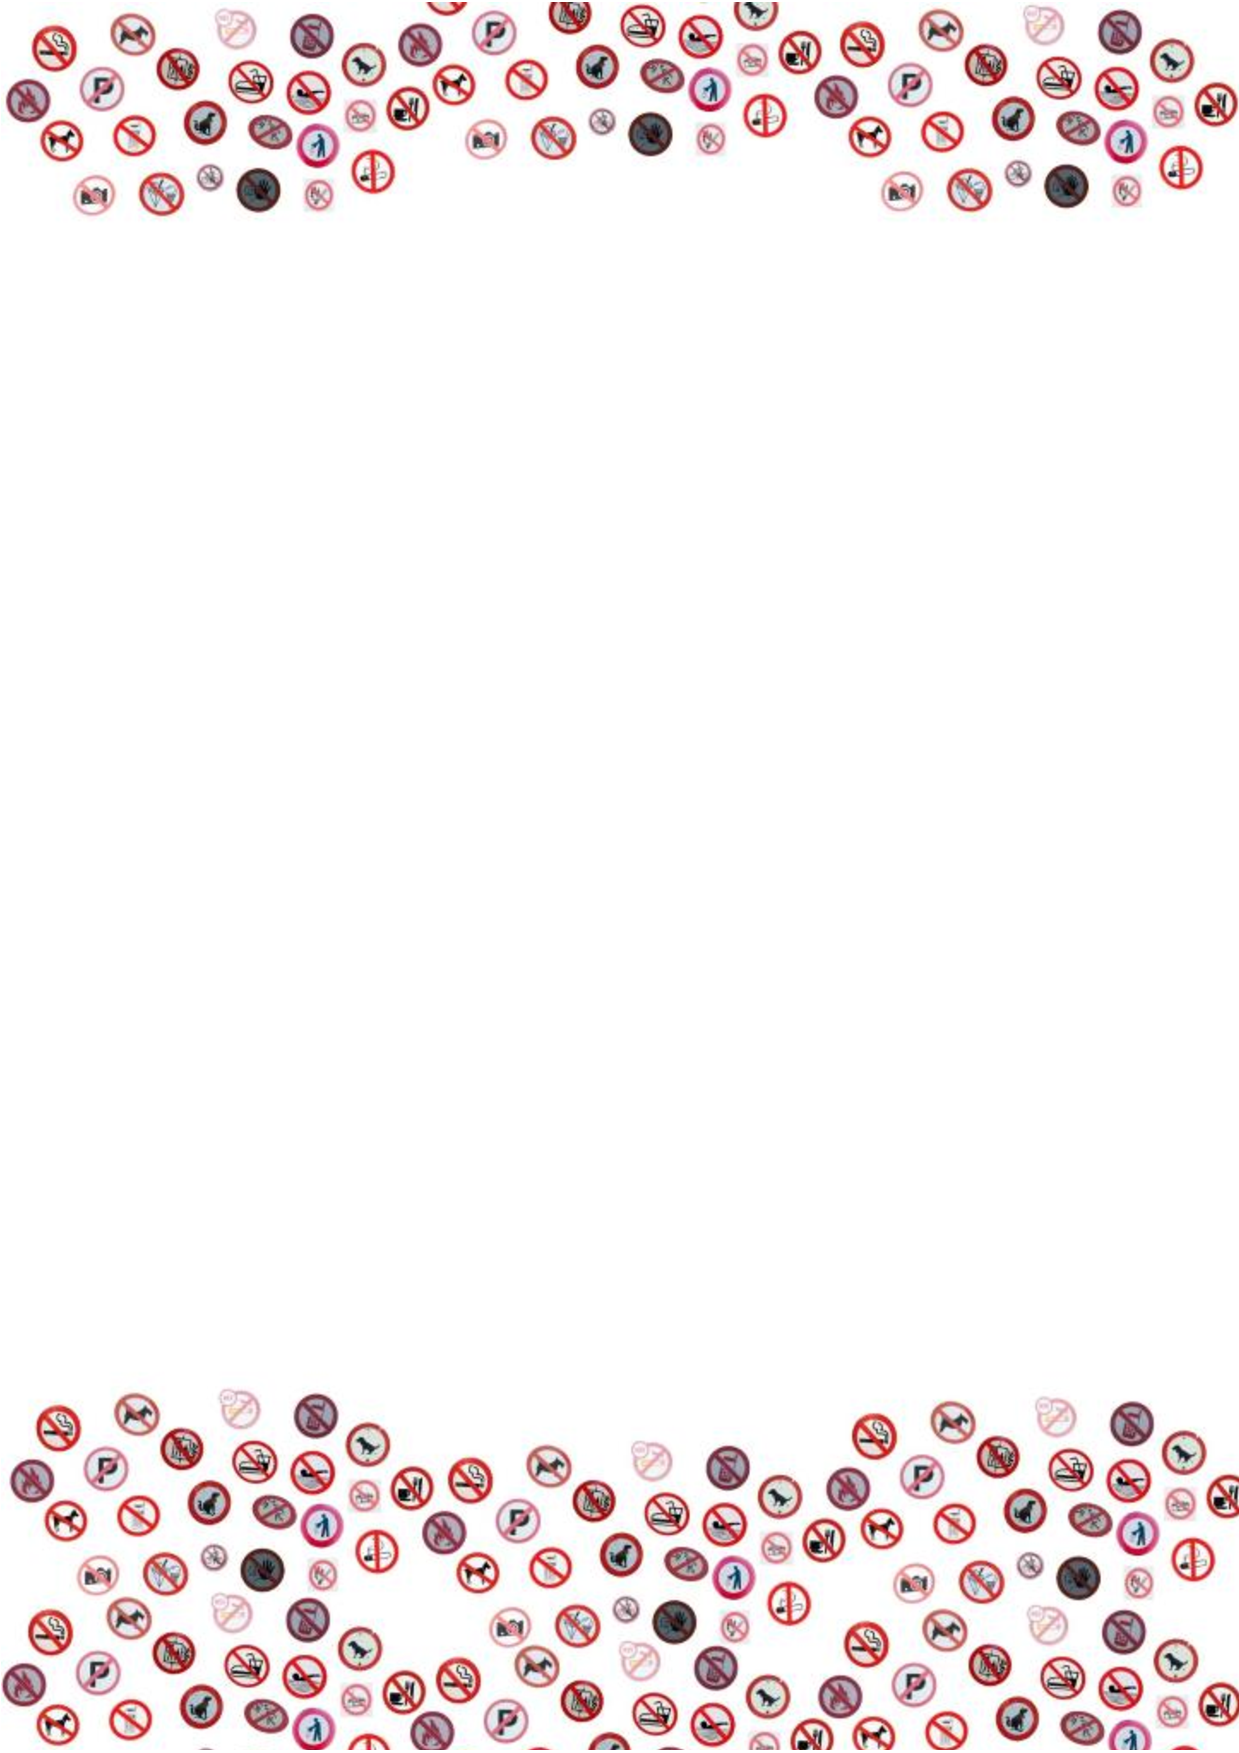
\includegraphics[scale=1]{bgschilder}}} % Image background
\centering
\vspace*{6cm}
\par\normalfont\fontsize{35}{35}\sffamily\selectfont

\includegraphics[width=\textwidth]{LogoWithName.jpg}
%\ProjectTitle\par % Book title
\vspace*{1cm}
{\Huge Manual}\par
\endgroup

%----------------------------------------------------------------------------------------
%	COPYRIGHT PAGE
%----------------------------------------------------------------------------------------

\newpage
~\vfill
\thispagestyle{empty}
Published \today

%\noindent Copyright \copyright\ 2013 John Smith\\ % Copyright notice

%\noindent \textsc{Published by Publisher}\\ % Publisher

%\noindent \textsc{book-website.com}\\ % URL

%\noindent Licensed under the Creative Commons Attribution-NonCommercial 3.0 Unported License (the ``License''). You may not use this file except in compliance with the License. You may obtain a copy of the License at \url{http://creativecommons.org/licenses/by-nc/3.0}. Unless required by applicable law or agreed to in writing, software distributed under the License is distributed on an \textsc{``as is'' basis, without warranties or conditions of any kind}, either express or implied. See the License for the specific language governing permissions and limitations under the License.\\ % License information

%\noindent \textit{First printing, March 2013} % Printing/edition date

%----------------------------------------------------------------------------------------
%	TABLE OF CONTENTS
%----------------------------------------------------------------------------------------

\chapterimage{Kollage.jpg} % Table of contents heading image

\pagestyle{empty} % No headers

\setcounter{tocdepth}{3}
\tableofcontents % Print the table of contents itself

\cleardoublepage % Forces the first chapter to start on an odd page so it's on the right

\pagestyle{fancy} % Print headers again

%----------------------------------------------------------------------------------------
%	Introduction
%----------------------------------------------------------------------------------------

\chapterimage{Kollage.jpg}
\chapter{Introduction to \ProjectTitle}
Welcome to isySUR (pronounce isy as ['i:zi]), a tool helping you to find the area of application of a space usage rule (SUR). For starting the command line version please see section \ref{sec:QuickstartTerminal}. For using the window version please read section \ref{sec:QuickstartWindow}. You can also run the window version on your android device. This is described in section \ref{sec:android}. For more details about the program see section \ref{sec:whatFor}.

\section{Quick start}
First decide if you like to use the command line version of \pt\ or if you prefer a graphical user interface. Please proceed with section \ref{sec:QuickstartTerminal} or section \ref{sec:QuickstartWindow} depending on your choice.

For installation instructions see section \ref{sec:installation}. For additional parameters see section \ref{sec:cli}.

For information about input and output file types see section \ref{sec:io}.

\subsection{\ProjectTitle\ in command line version}\label{sec:QuickstartTerminal}
For the command line version type
\begin{verbatim}
	$ python run_isySUR.py cli [-h] [-c CONFIG] input output
\end{verbatim}
where \texttt{input} is the path to the input file containing the SURs which areas of influence should be computed and \texttt{output} is the path for the resulting area(s) of influence. If the path points to a file, only one KML file will be created, containing all calculated areas. If the path points to a directory a KML file for each SUR will be created as well as one containing all areas.

\subsection{\ProjectTitle\ in window version}\label{sec:QuickstartWindow}
For the window version just type
\begin{verbatim}
	$ python run_isySUR.py gui [-h] [-c CONFIG]
\end{verbatim}
In Menu you find the possibility to load a SUR input file. After calculating you can save the area(s) of application.

\section{What is \ProjectTitle?}\label{sec:whatFor}
\begin{figure}
\centering
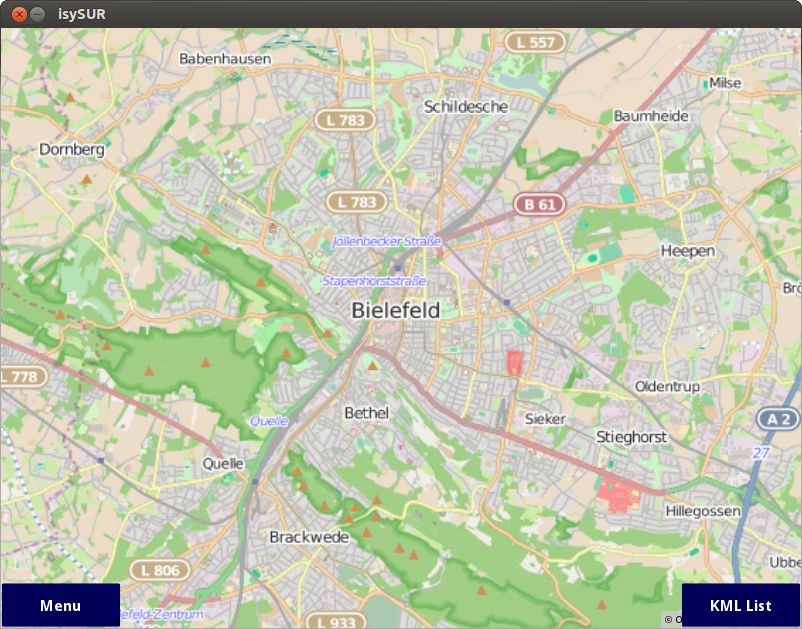
\includegraphics[width=0.75\textwidth]{screenshot.png}
\caption{\pt\ in GUI version}
\end{figure}
\pt\ is a program that tries to calculate the intuitive area of application of a space usage rule by its coordinates and data from OpenStreetMap\footnote{\url{http://www.openstreetmap.org}}. It was developed as part of the informatiCup, a programming competition for students organized by the German Informatics Society (Gesellschaft für Informatik e.V.). Our team is called ISY and consists of Adriana-Victoria Dreyer, Jacqueline Hemminghaus, Jan Pöppel and Thorsten Schodde, four students of the master study course `Intelligent Systems' at Bielefeld University.

Using \pt\ is very easy. You give an input file with the coordinates of the SURs and the intended area of application is computed. Optionally, you can add a configuration file that classifies SURs in those that are applicable only indoor, those that are applicable only outdoor or those that are applicable indoor as well as outdoor (both) to get a better result. In the GUI version the calculated areas are shown on a map and you can choose which ones you want to be displayed. They can be saved into a file to reload them whenever you want to have a look at them.

\section{Content of \ProjectTitle}
In the archive you can find the following data (bold printed files will be installed with the install command):
\begin{itemize}
	\item data (directory) - examples for space usage rules\footnote{see section \ref{sec:surs}}
	\item doc (directory) - documentation directory
	\begin{itemize}
		\item manual.pdf - this manual
		\todol{add pydoc}
	\end{itemize}
	\item \textbf{isySUR} (directory) - the source files for the isySUR Python package
	\begin{itemize}
		\item \textbf{gui} (directory) - source files for GUI version
		\item tests (directory) - \pt\ was developed using test driven development. In this directory you will find the test files.
	\end{itemize}
	\item testData (directory) - data for tests and test data sets
	\begin{itemize}
		\item dataOnlyForTests (directory) - Some of the test files need data that is stored in this directory
		\item Data.txt - a possible input file
	\end{itemize}
	\item README.txt
	\item \textbf{run\_isySUR.py} - the Python script to run \pt
	\item run\_tests.py - script that runs all or some tests in isySUR/tests/, used for development
	\item setup.py - the setup script to install \pt
	\item surConfig.cfg - a configuration file that can optionally be used for computation\footnote{see section \ref{sec:usage}}
\end{itemize}


%----------------------------------------------------------------------------------------
%	Using the program
%----------------------------------------------------------------------------------------

\chapter{Using \ProjectTitle}
In this chapter the usage of \pt\ is described in detail. First you can find installation instructions in section \ref{sec:installation}, detailed usage instruction for both program versions are following in section \ref{sec:usage}.

\section{Requirements and installation}\label{sec:installation}
\pt\ is written in Python so you get a Python script, which starts the main program, and a package with the tools. For running the command line version you do not need much more than basic Python. If you prefer to use a graphical user interface you will have to install some more packages.
\subsection{Requirements}\label{sec:requirements}
\begin{enumerate}
	\item \textbf{basic requirements:}
	\begin{itemize}
		\item Python 2.7
		\item requests (HTTP library)
		\item internet connection
	\end{itemize}
	~\\
	To run a Python script you need Python. Python comes with most Linux distributions. For the use on Windows machines you will have to install Python manually\footnote{get Python here: \url{https://www.python.org}}. \pt\ uses data from OpenStreetMap\footnote{\url{http://www.openstreetmap.org}} to calculate the area of application. Therefore an internet connection is required. The data transfer in Python is realised with the requests\footnote{\url{http://docs.python-requests.org}\label{fn:requests}} library. You can easily install it using pip\footnote{\url{https://pip.pypa.io}}, a Python installation tool
	\begin{verbatim}
		$ pip install requests
	\end{verbatim}
	or see requests web page\footref{fn:requests}.
	\newpage
	\item \textbf{additional requirements for the GUI version:}
	\begin{itemize}
		\item Kivy
		\item concurrent.futures
	\end{itemize}
	For the graphical user interface Kivy is used. Kivy\footnote{\url{http://kivy.org}} is a cross-platform Python Framework for NUI Development. For installation on Ubuntu we recommend the installation with apt-get as described on their web page. For use on Windows and starting Kivy applications from the command line we recommend to install Kivy and pygame (needed for Kivy) with the unofficial precompiled binaries\footnote{Kivy: \url{http://www.lfd.uci.edu/\%7Egohlke/pythonlibs/\#kivy}}\footnote{pygame: \url{http://www.lfd.uci.edu/\%7Egohlke/pythonlibs/\#pygame}}. On MacOSX the easiest way to run Kivy applications, like \pt, is with the Kivy launcher as mentioned on the Kivy web site\footnote{\url{http://kivy.org/docs/installation/installation-macosx.html}}.
	
On all OS futures can be installed via pip
\begin{verbatim}
	$ pip install futures
\end{verbatim}
\end{enumerate}

\subsection{Installation}
You have got an archive of type .tar.gz. Please unpack the archive into a directory of your choosing. Because \pt\ is a Python script you do not need to install it. It is also possible to install only the dependencies and run \pt\ by typing from within the directory you chose before:
\begin{verbatim}
	$ python run_isySUR.py [parameters]
\end{verbatim}
~\\

For installing the script and tool package browse the directory you chose and install \pt\ with the help of Python's distutils:
\begin{verbatim}
	$ python setup.py install
\end{verbatim}
Now you are able to start \pt\ any time and anywhere by typing:
\begin{verbatim}
	$ run_isySUR.py [parameters]
\end{verbatim}

\section{Input and output}\label{sec:io}
The input of the space usage rules was specified in the programming task as well as the output in .kml format. For more information about the decision to add a configuration file please see section \ref{sec:data_usage}.

\subsection{Space usage rules}
The SUR file is a plain text file. The first line holds the number of lines in the file, that will be used for constructing SURs, which are to be computed. The following lines represent the rules. A line must always start with the SUR id, followed by the latitude and longitude coordinates of the rule. The last entry is a brief description of the rule. The entries are comma separated. Decimal separator in latitude and longitude is a point. One SUR id can span several consecutive lines in order to add several rules to the same SUR.
\newpage
Example file:
\begin{verbatim}
3
0061, 50.9304, 5.34470, smoking="no"
0061, 50.9304, 5.34470, access:dog="no"
0062, 50.9306, 5.34366, smoking="no"
\end{verbatim}

\subsection{Configuration file}\label{sec:confinput}
The configuration file is a plain text file. In this file one or more blocks starting with `[Indoor]', `[Outdoor]' or `[Both]' are found. After these headlines the names of the rules follow that belong to these categories of area of influence.
\\~

Example file:
\begin{verbatim}
[Indoor]
access:age="21+"
camera="no"
[Outdoor]
fishing="no"
littering="no"
[Both]
access:dog="no"
open_fire="no"
\end{verbatim}

These configuration files can be used to adapt the area calculation to better suite local space usage rule customs. For more details about how these categories influence the calculation see section \ref{sec:data_usage}.

\subsection{Keyhole Markup Language}
Output files are in .kml format where KML stands for Keyhole Markup Language. For syntax definition and documentation please visit \url{https://developers.google.com/kml}. Kml version 2.1 is used for the produced output files.

The GUI version provides also the possibility to read KML files to display the areas. For this KML version 2.1 as well as 2.2 is supported.

\section{Command line and GUI version}\label{sec:usage}
\pt\ comes with two versions: One for command line use and another one for users who prefer to use a graphical user interface.
For using the command line interface type:
\begin{verbatim}
	$ run_isySUR.py cli [parameters]
\end{verbatim}
For using the graphical user interface type:
\begin{verbatim}
	$ run_isySUR.py gui [parameters]
\end{verbatim}

Notice that the GUI version has more requirements than the command line version. See \ref{sec:requirements} for more details.

\subsection{Command line version}\label{sec:cli}
Usage of the command line version:
\begin{verbatim}
	$ run_isySUR.py cli [-h] [-c CONFIG] input output
\end{verbatim}

\subsubsection{Parameters}
The parameters of \texttt{run\_isySUR.py cli} (bold arguments are required):
\begin{itemize}
	\item \textbf{input} - Path to the input file containing the SURs. See \ref{sec:io} for the required format.
	\item \textbf{output} - Path where to put the output file(s). If this path points to a file, a single output .kml-file containing all computed areas is created. If it points to a directory, one .kml-file for each SUR is created in this directory as well as one .kml-file containing all computed areas.
	\item -c CONFIG (--config CONFIG) - With this parameter an optional config file with SUR classifications (indoor, outdoor, both) is used for computation. For the format of the file see \ref{sec:io}.
	\item -h - If this parameter is given, a short help message containing all parameters is shown.
\end{itemize}

\subsection{GUI version}\label{sec:gui}
\todol{add information with config - first safe, afterwards it will be applied}
Usage of the GUI version:
\begin{verbatim}
	$ run_isySUR.py gui [-h] [-c CONFIG]
\end{verbatim}
~\\
If you do not want to give parameters you can also start the GUI version with
\begin{verbatim}
	$ run_isySUR.py
\end{verbatim}
or a simple double click on the file (when .py-files are connected to python). When the GUI cannot be loaded, the command line version is started.

When the GUI version could not be started, e.g. because of missing requirements, you can proceed with the command line version. You will be asked for an input file and an output path, to run the program. If you do not want to use this version you can type \texttt{'exit'} to exit the program.

\subsubsection{Parameters}
The parameters of \texttt{run\_isySUR.py gui}:
\begin{itemize}
	\item -c CONFIG (--config CONFIG) - With this parameter an optional config file with SUR classifications (indoor, outdoor, both) is used for computation. For the format of the file see \ref{sec:io}.
	\item -h - If this parameter is given, a short help message containing all parameters is shown.
\end{itemize}

\subsubsection{The menu}
\begin{figure}
\centering
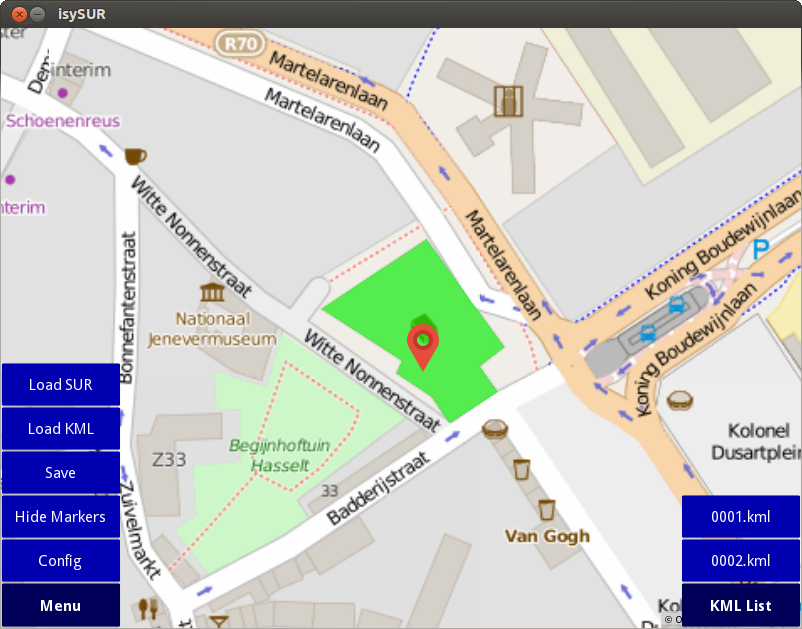
\includegraphics[width=0.75\textwidth]{GUI.png}
\caption{GUI with open menu and KML list}
\end{figure}
On the left side you can find the menu that holds the functionality you can use. In the menu you will find the following possibilities:
\begin{itemize}
	\item \textbf{Load SUR} - Choose the file with the coordinates of your SURs. See section \ref{sec:io} for more information about the format. The area of application of the SURs will be calculated. An information text will inform you about the ID of the current SUR. When the KML list is open you can see that areas are added. Calculated areas are displayed on the map as well as red markers at the SUR's coordinates. After a calculation is finished you can start another one. The new areas will be added to the ones already in the KML list.
	\item \textbf{Load KML} - Choose some KML file you have already saved during the last usage. Or maybe you made your own KML file with another program. See section \ref{sec:io} for more information about the format. The areas contained in your file are displayed on the map and an entry for this file is added to those already in the KML list.
	\item \textbf{Save KML} - All KMLs that are currently selected in the KML list are saved to the file or folder that you can choose here.
	\item \textbf{SUR Position} - The red SUR markers can be hidden and shown with this button.
	\item \textbf{Config} - With this button you can open the configuration window. If you used the \texttt{--config} parameter there is already a configuration file loaded. You can load another configuration file, add or remove some rules and save your personal configuration file. With your configuration you say if you prefer to find an area for a SUR indoor or outdoor or if you think that kind of rule can be applicable indoor as well as outdoor. The following computations will use the new configuration.
\end{itemize}

\subsubsection{KML list}
On the right side of the window, there is the KML list. This list tells you which areas you have calculated or loaded. You can scroll the list if it is too long for the window with the mouse wheel or by dragging it with the mouse. When you click on an entry which area is not in view the map will jump to that area. When you click on an entry which area is already in view you can hide it. Hidden areas are not saved into a KML file. With another click you can make an area visible again.

\subsection{Using android}\label{sec:android}
Of course calculating SURs at home is nice but in general you would like to know the area of application a space usage rule standing in front of it. This is possible on your android device (with internet connection). In the archive you can find the isySUR\todo{name of file correct?}.apk that you can install on your device. Just copy it on the device e.g. via USB and enable the device option to install from unknown sources. Browsing to the .apk and clicking on it starts the installation. After that you will find isySUR in your apps and can use it exactly like the GUI version described in section \ref{sec:gui}.

%----------------------------------------------------------------------------------------
%	Technical and implementation details
%----------------------------------------------------------------------------------------

\chapter{Technical and implementation details}
In this chapter you will gain an insight into the development and learn some implementation details. The implemented algorithm to calculate the intended areas of application is explained in section \ref{sec:algorithm}. After that an evaluation of the achieved results follows in section \ref{sec:evaluation}.

\todol{Code documentation -> pydoc?}

\section{Development}
For this project we decided to use Python. First of all, we all wanted to challenge and expand upon our Python knowledge. Furthermore Python is mostly OS independent and can even be ported to android for portable usage which seems to be a good feature here.

This project was created using test driven development on the unittest layer. This does not only allow us to keep track of unwanted side effects of new functionality, but also helps assigning work load to the different members, because it can be easier to write a failing unittest with a bit of information, that is assigned to someone, than it is to explain all the requirements for some new functionality.

\pt\ was created in two steps: First the command line version was created and the first versions of the algorithm were implemented. While the algorithm was improved and reworked, it was decided to add a GUI because a lightweight tool for displaying the calculated areas was missing. Furthermore, it helped in improving the algorithm by enabling rapid testing of changes. On top of that, not all people like to use a command line tool.

For the GUI the Kivy framework is used. We base the display of the OSM map on mapview from the Kivy Garden\footnote{see \url{https://github.com/kivy-garden/garden.mapview}} which we adapted to suit our needs.

At the beginning of the project the idea of an app came up and with the Kivy framework for the GUI the foundations for this was laid. With buildozer\footnote{see \url{https://github.com/kivy/buildozer}} a nice tool for packaging an apk file from our project was found.

\subsection{Data usage}\label{sec:data_usage}
In the competition intended to use as input is the SUR file as well as photos of the real signs belonging to the space usage rules. We deliberately do not use the images in our analysis. This is because they do not give us reliable information about the interesting polygons. The variety of possible signs, including totally unknown ones, (and their placement in/on/around the intended area) make it infeasible to perform robust image recognition or classification. Furthermore the only relevant information we think one could extract from images, refers to an inside/outside classification of the rule. However, even this classification would not be reliable and robust enough in the general use case.

One might consider using images and compute vision techniques in the future, when the Google StreetView recordings cover virtually everything and these images are available to this program as well, but until then we do not believe we can extract useful information from the images.

We do allow the usage of the rule types/names (e.g. access:21="no") to some minimal extend. We allow config files (see \ref{sec:confinput} for details about the format) that classify the rules to be applicable indoor, outdoor or indoor as well as outdoor (both). We use these classifications to narrow down the possible OSM elements around the target coordinates. Unknown rules will always get the ``both'' classification so that we do not ignore relevant information in those cases. We hope to improve our results, by complying with local space usage rule customs, and reduce computational costs by doing so. However, in a general context most rules are applicable indoors as well as outdoors, which means that these classifications will most likely only be useful in individual cases. 

\subsection{Data structure}
In order to be able to work freely with all the data that we require when computing suitable areas for SURs we have introduced our own data structure.
\begin{itemize}
	\item sur: A wrapper object for the SURs. It enables us to handle the file only once at the beginning.
	\item osmData: Wrapper for the OSM elements Node, Way and Relation. We convert the xml data we receive from OSM to these objects, so that we do not have to work on the xml for computation.
	\item kmlData: Wrapper objects for a KML and included placemarks. These will be created by our algorithm and can be saved to a .kml file.
\end{itemize}

Furthermore, our data structure splits our program into nice modular chunks that can be reused independently in other project if desired.

\section{Algorithm}\label{sec:algorithm}
\todol{pseudocode}
\todol{rework this section}

Our main focus lies upon the coordinate of the SUR. In a bounding box (currently 100m\todo{this is not up to date is it?} might be reduced further) around the given coordinates, we start by searching for the closest OSM relations and ways (we omit nodes for now, since they hardly provide any connectivity information, necessary to be able to construct reasonable polygons). We use a bounding box of limited size because we want to reduce the amount of data that we need to request from OSM and we work on the assumption that these coordinates should always relatively close to the intended area. Unfortunately some coordinates (at least in the test data) are quite far away from the intended area, which can lead to finding unintended polygons that are closer to the coordinates. Furthermore the OSM data is not complete and even some elements from the test data are not present in OSM, which means, that we have no way of ever finding the intended polygon.

\section{Evaluation}\label{sec:evaluation}
\todol{Berechnen Sie nun die Geltungsbereiche der Space Usage Rules aus Ihrer Umgebung mit Ihrer Implementierung aus der ersten Runde.
Diskutieren Sie die Korrektheit und die Präzision der von Ihnen berechneten Lösungen für die Space
Usage Rules des Testdatensatzes und denen aus Ihrer Umgebung. Vergleichen Sie dazu die berechneten mit den intuitiv beabsichtigten Geltungsbereichen.}

\section{Further Work}
Our major focus of future work will be the development of the GUI. Most of all we like to implement a possibility to list up all placemarks of one KML similar to Google Earth, so that the user can jump to every placemark on the map he or she likes and not only to the last one of each KML. Furthermore the user should be able to display the rules that are applied in any polygon when clicking on it.
Another improvement of the GUI should be the opportunity to load several KMLs at once, because currently the user can only load one KML file at a time.

For a better usability on mobile devices it should be implemented that a click anywhere on the map adds a new SUR and the program calculates the corresponding area. Also the use on mobile devices shows that the memory requirements should be improved.

To improve the calculation of our KMLs we think about using multiple data sources because OpenStreetMap sometimes has a lack of data information.

In order to improve \pt\ and make it available for others, we are going to make our repository public after the competition.

%----------------------------------------------------------------------------------------
%	Own SURs
%----------------------------------------------------------------------------------------

\chapter{Added SURs}\label{sec:surs}
For the competition at least ten new space usage rules should be found. Here our 20 found SURs are presented.

\newcommand{\sur}[3]{\begin{minipage}{0.2\linewidth}
	\centering
	\includegraphics[width=\linewidth]{surs/#1}
	#2: #3
\end{minipage}}
\newcommand{\area}[2]{\begin{minipage}{0.2\linewidth}
	\centering
	\includegraphics[width=\linewidth]{intuitive_areas/#1}
	intuitive area of #2
\end{minipage}}

\begin{tabular}{cccc}
\sur{isy0001.jpg}{isy0001.jpg}{smoking="no"} & \area{isy0001.png}{isy0001.jpg} & \sur{isy0002.jpg}{isy0002.jpg}{smoking="no", access:dog="no"} & \area{isy0002.png}{isy0002.jpg} \\ 
~\\
\hline
~\\
\sur{isy0003.jpg}{isy0003.jpg}{access:dog="no"} & \area{isy0003.png}{isy0003.jpg} & \sur{isy0004.jpg}{isy0004.jpg}{smoking="no"} & \area{isy0004.png}{isy0004.jpg}
\end{tabular}

\begin{tabular}{cccc}
\sur{isy0005.jpg}{isy0005.jpg}{smoking="no"} & \area{isy0005.png}{isy0005.jpg} & \sur{isy0006.jpg}{isy0006.jpg}{smoking="no"} & \area{isy0006.png}{isy0006.jpg} \\
~\\
\hline
~\\
\sur{isy0007.jpg}{isy0007.jpg}{smoking="no"} & \area{isy0007.png}{isy0007.jpg} & \sur{isy0008.jpg}{isy0008.jpg}{smoking="no"} & \area{isy0008.png}{isy0008.jpg} \\
~\\
\hline
~\\
\sur{isy0009.jpg}{isy0009.jpg}{smoking="no", access:bicycle="no"} & \area{isy0009.png}{isy0009.jpg} & \sur{isy0010.jpg}{isy0010.jpg}{access:bicycle="no"} & \area{isy0010.png}{isy0010.jpg} \\
~\\
\hline
~\\
\sur{isy0011.jpg}{isy0011.jpg}{access="no"} &\area{isy0011and12.png}{isy0011.jpg}  & \sur{isy0012.jpg}{isy0012.jpg}{access:pram="no"} & \area{isy0011and12.png}{isy0012.jpg}
\end{tabular}

\begin{tabular}{cccc}
\sur{isy0013.jpg}{isy0013.jpg}{smoking="no"} & \area{isy0013.png}{isy0013.jpg} & \sur{isy0014.jpg}{isy0014.jpg}{smoking="no", noise="no"} & \area{isy0014.png}{isy0014.jpg} \\
~\\
\hline
~\\
\sur{isy0015.jpg}{isy0015.jpg}{smoking="no", access:dog="no"} & \area{isy0015.png}{isy0015.jpg} & \sur{isy0016.jpg}{isy0016.jpg}{access:fire\_case="no"} & \area{isy0016.png}{isy0016.jpg} \\
~\\
\hline
~\\
\sur{isy0017.jpg}{isy0017.jpg}{dog\_waste="no"} & \area{isy0017.png}{isy0017.jpg} & \sur{isy0018.jpg}{isy0018.jpg}{smoking="no"} & \area{isy0018.png}{isy0018.jpg} \\
~\\
\hline
~\\
\sur{isy0019.jpg}{isy0019.jpg}{access:bicycle="no"} & \area{isy0019.png}{isy0019.jpg} & \sur{isy0020.jpg}{isy0020.jpg}{access:dog="no", access:skate="no"} & \area{isy0020.png}{isy0020.jpg}
\end{tabular}

%----------------------------------------------------------------------------------------
%	List of TODOS
%----------------------------------------------------------------------------------------

\listoftodos  %to be deleated in the end

\end{document}
